\paragraph{GET /:lang/user/:userId/search/:keyword/users}
\begin{itemize}
\item \textbf{Successo}
Questo scenario rappresenta la ricerca da parte di utente di altri utenti; verrà ritornata la lista degli utenti il cui username contiene la keyword inserita nella barra di ricerca. 

\begin{figure}[ht]
	\centering
	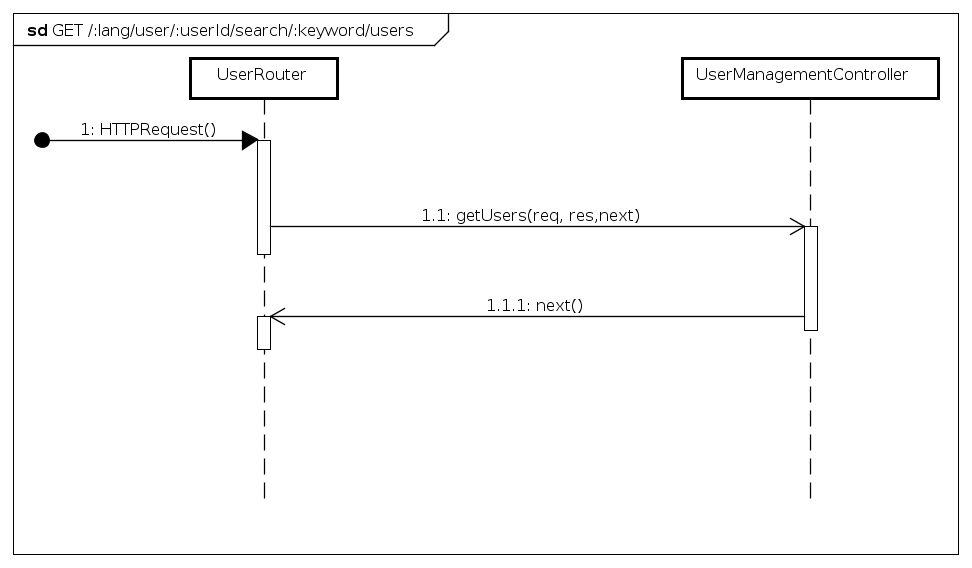
\includegraphics[scale=0.45]{UML/DiagrammiDiSequenza/Back-end/GET__lang_user__userId_search__keyword_users_success.png}
	\caption{Successo: GET /:lang/user/:userId/search/:keyword/users}
\end{figure}
\FloatBarrier

\item \textbf{Fallimento}
Questo scenario rappresenta una ricerca da parte di un utente di altri utenti non andata a buon fine; in questo caso il modulo \texttt{UserManagementController} ritornerà un \texttt{next(err)} al router che avrà il compito di reinstradarlo (indirizzandolo verso \texttt{ErrorHandler}).

\begin{figure}[ht]
	\centering
	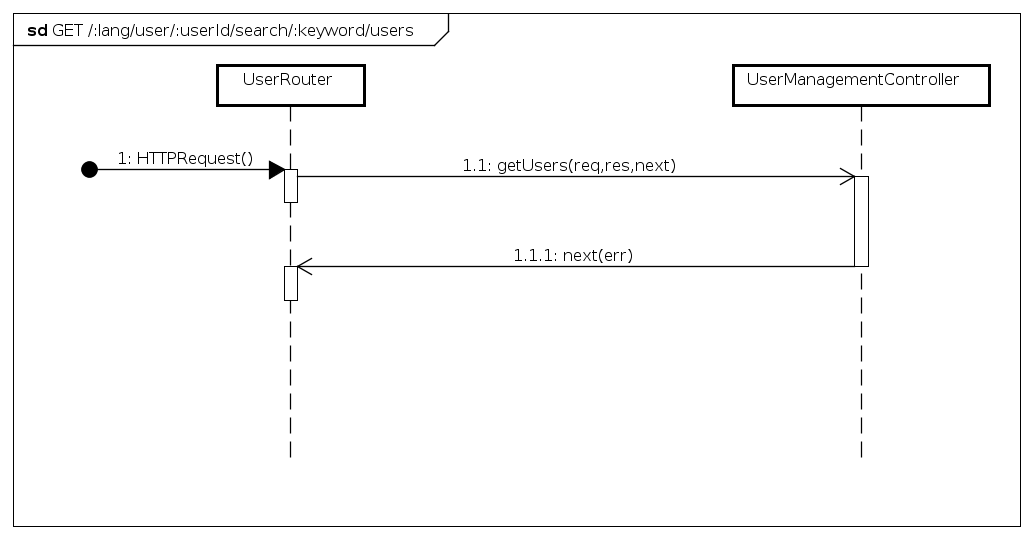
\includegraphics[scale=0.45]{UML/DiagrammiDiSequenza/Back-end/GET__lang_user__userId_search__keyword_users_failure.png}
	\caption{Fallimento: GET /:lang/user/:userId/search/:keyword/users}
\end{figure}
\FloatBarrier

\end{itemize}






\paragraph{GET /:lang/user/:userId/search/:keyword/quizzes}
\begin{itemize}
\item \textbf{Successo}
Questo scenario rappresenta la ricerca da parte di utente di questionari; verrà ritornata la lista dei questionari il cui titolo contiene la keyword inserita nella barra di ricerca.

\begin{figure}[ht]
	\centering
	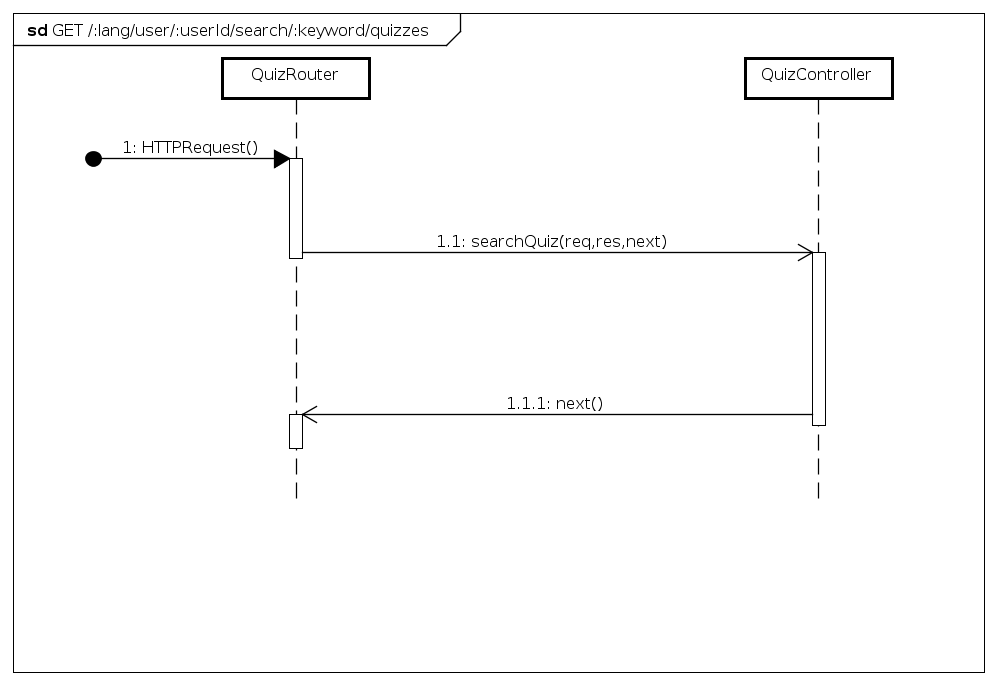
\includegraphics[scale=0.45]{UML/DiagrammiDiSequenza/Back-end/GET__lang_user__userId_search__keyword_quizzes_success.png}
	\caption{Successo: GET /:lang/user/:userId/search/:keyword/quizzes}
\end{figure}
\FloatBarrier

\item \textbf{Fallimento}
Questo scenario rappresenta una ricerca da parte di un utente di questionari non andata a buon fine; in questo caso il modulo \texttt{QuizController} ritornerà un \texttt{next(err)} al router che avrà il compito di reinstradarlo (indirizzandolo verso \texttt{ErrorHandler}).

\begin{figure}[ht]
	\centering
	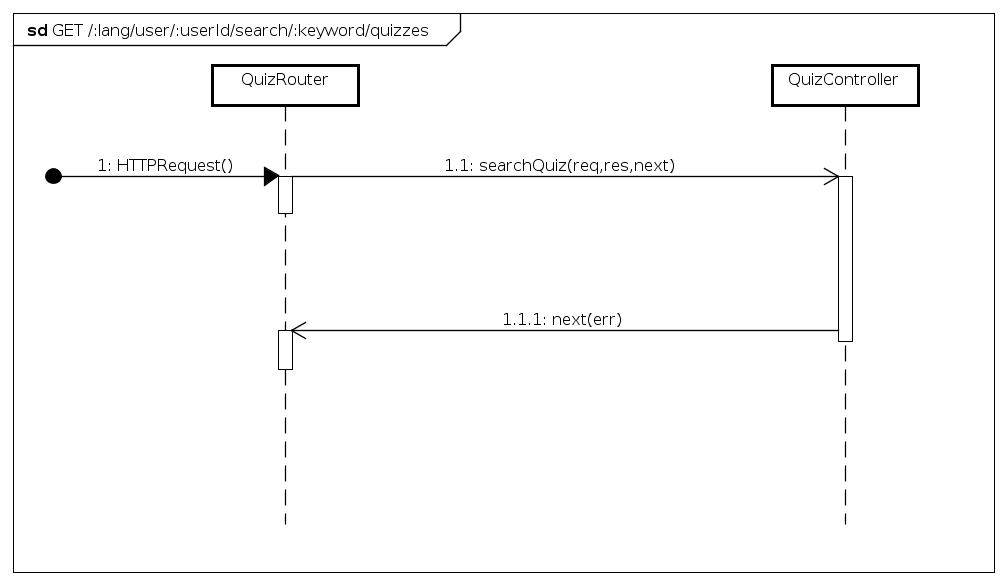
\includegraphics[scale=0.45]{UML/DiagrammiDiSequenza/Back-end/GET__lang_user__userId_search__keyword_quizzes_failure.png}
	\caption{Failure: GET /:lang/user/:userId/search/:keyword/quizzes}
\end{figure}
\FloatBarrier
\end{itemize}






\paragraph{GET /:lang/user/:userId/search/users/:users}
\begin{itemize}
\item \textbf{Successo}
Questo scenario rappresenta la visualizzazione di un utente tra quelli ritornati come risultato della ricerca; verranno visualizzate le informazioni riguardanti l'utente selezionato.

\begin{figure}[ht]
	\centering
	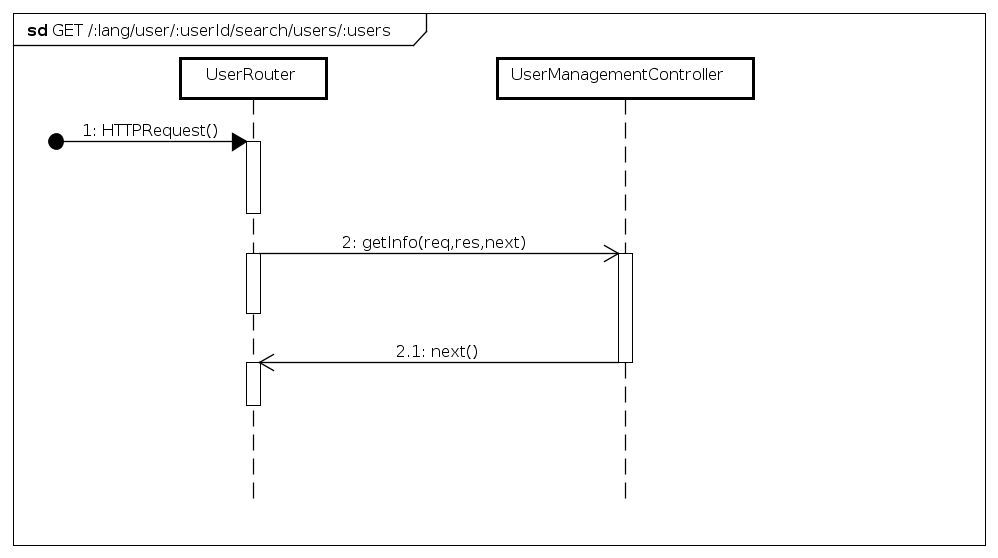
\includegraphics[scale=0.45]{UML/DiagrammiDiSequenza/Back-end/GET__lang_user__userId_search_users__users_success.png}
	\caption{Successo: GET /:lang/user/:userId/search/users/:users}
\end{figure}
\FloatBarrier

\item \textbf{Fallimento}
Questo scenario rappresenta la visualizzazione delle informazioni di un utente non andata a buon fine; in questo caso il modulo \texttt{UserManagementController} ritornerà un \texttt{next(err)} al router che avrà il compito di reinstradarlo (indirizzandolo verso \texttt{ErrorHandler}).

\begin{figure}[ht]
	\centering
	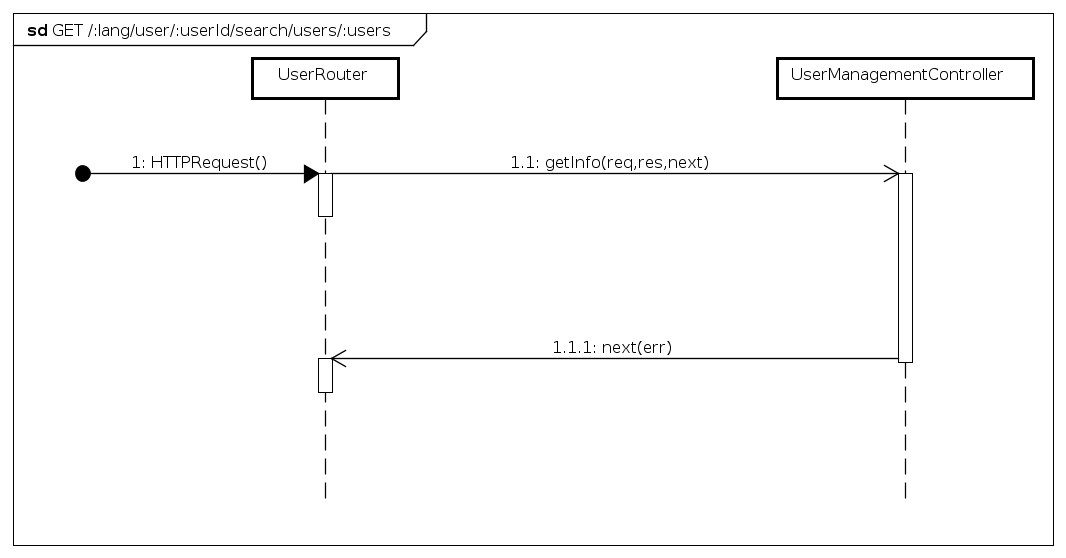
\includegraphics[scale=0.45]{UML/DiagrammiDiSequenza/Back-end/GET__lang_user__userId_search_users__users_failure.png}
	\caption{Fallimento: GET /:lang/user/:userId/search/users/:users}
\end{figure}
\FloatBarrier

\end{itemize}





\paragraph{GET /:lang/user/:userId/search/quizzes/:quizId}
\begin{itemize}
\item \textbf{Successo}
Questo scenario rappresenta la visualizzazione di un questionario tra quelli ritornati come risultato della ricerca.

\begin{figure}[ht]
	\centering
	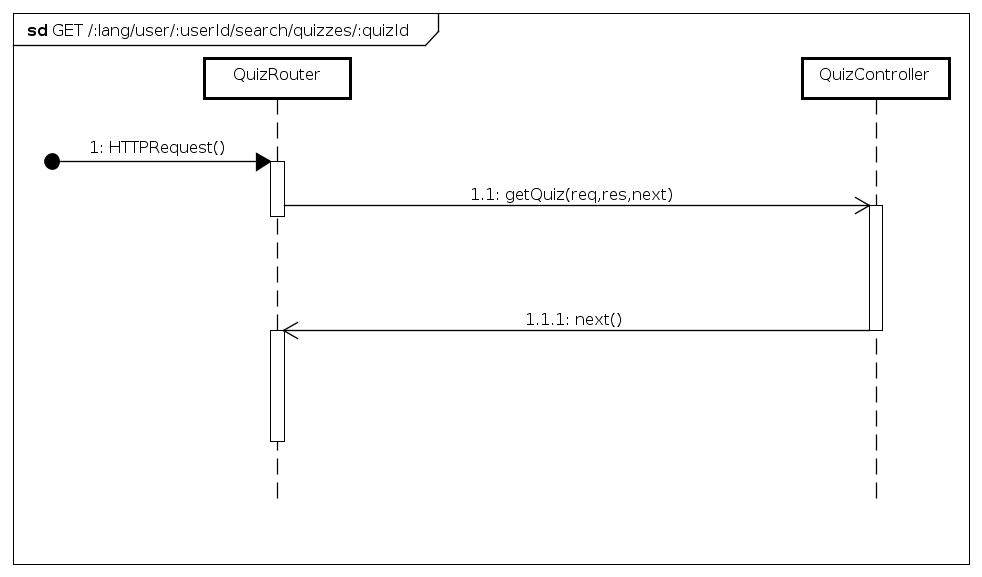
\includegraphics[scale=0.45]{UML/DiagrammiDiSequenza/Back-end/GET__lang_user__userId_search_quizzes__quizId_success.png}
	\caption{Successo: GET /:lang/user/:userId/search/quizzes/:quizId}
\end{figure}
\FloatBarrier

\item \textbf{Fallimento}
Questo scenario rappresenta la visualizzazione di un questionario non andata a buon fine; in questo caso il modulo \texttt{QuizController} ritornerà un \texttt{next(err)} al router che avrà il compito di reinstradarlo (indirizzandolo verso \texttt{ErrorHandler}).

\begin{figure}[ht]
	\centering
	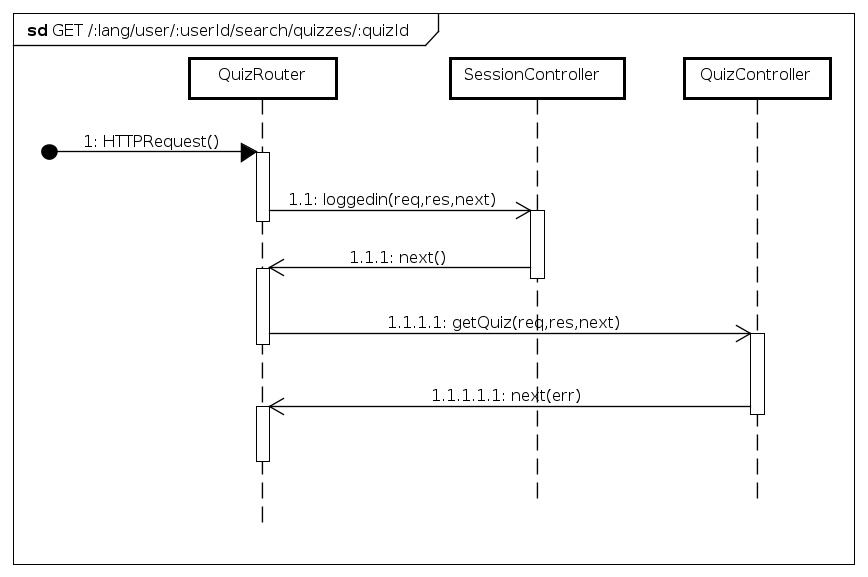
\includegraphics[scale=0.45]{UML/DiagrammiDiSequenza/Back-end/GET__lang_user__userId_search_quizzes__quizId_failure.png}
	\caption{Fallimento: GET /:lang/user/:userId/search/quizzes/:quizId}
\end{figure}
\FloatBarrier

\end{itemize}
